% mnras_template.tex
%
% LaTeX template for creating an MNRAS paper
%
% v3.0 released 14 May 2015
% (version numbers match those of mnras.cls)
%
% Copyright (C) Royal Astronomical Society 2015
% Authors:
% Keith T. Smith (Royal Astronomical Society)

% Change log
%
% v3.0 May 2015
%    Renamed to match the new package name
%    Version number matches mnras.cls
%    A few minor tweaks to wording
% v1.0 September 2013
%    Beta testing only - never publicly released
%    First version: a simple (ish) template for creating an MNRAS paper

%%%%%%%%%%%%%%%%%%%%%%%%%%%%%%%%%%%%%%%%%%%%%%%%%%
% Basic setup. Most papers should leave these options alone.
%\documentclass[a4paper,fleqn,usenatbib]{mnras}
\documentclass[a4paper,fleqn,usenatbib,useAMS]{mnras}
% MNRAS is set in Times font. If you don't have this installed (most LaTeX
% installations will be fine) or prefer the old Computer Modern fonts, comment
% out the following line
% Depending on your LaTeX fonts installation, you might get better results with one of these:
\usepackage{mathptmx}


% Use vector fonts, so it zooms properly in on-screen viewing software
% Don't change these lines unless you know what you are doing
\usepackage[T1]{fontenc}
\usepackage{ae,aecompl}


%%%%% AUTHORS - PLACE YOUR OWN PACKAGES HERE %%%%%

% Only include extra packages if you really need them. Common packages are:
\usepackage{graphicx}	% Including figure files
\usepackage{amsmath}	% Advanced maths commands
\usepackage{amssymb}	% Extra maths symbols

%%%%%%%%%%%%%%%%%%%%%%%%%%%%%%%%%%%%%%%%%%%%%%%%%%

%%%%% AUTHORS - PLACE YOUR OWN COMMANDS HERE %%%%%

\usepackage{times}
\usepackage{epstopdf}
\usepackage{graphicx}
\usepackage{txfonts}
\usepackage{natbib}
\usepackage{array}
\setlength{\topmargin}{-1.2cm}

% Please keep new commands to a minimum, and use \newcommand not \def to avoid
% overwriting existing commands. Example:
%\newcommand{\pcm}{\,cm$^{-2}$}	% per cm-squared

%%%%%%%%%%%%%%%%%%%%%%%%%%%%%%%%%%%%%%%%%%%%%%%%%%

%%%%%%%%%%%%%%%%%%% TITLE PAGE %%%%%%%%%%%%%%%%%%%

% Title of the paper, and the short title which is used in the headers.
% Keep the title short and informative.
\title[Beware the effect of edge-on discs]{SHARP - II: Revealing a bias in observational measurements of dark matter substructure with gravitational lens flux ratios}
\author[Hsueh et al.]{J.-W. Hsueh,$^{1}$\thanks{E-mail: jwhsueh@ucdavis.edu} C. D. Fassnacht,$^{1}$ S. Vegetti,$^{2}$  J. P. McKean,$^{3,4}$ C. Spingola,$^{4}$ M. W. Auger,$^{5}$
\newauthor  L. V. E. Koopmans,$^{4}$ and D. J. Lagattuta$^{6}$\\
$^{1}$Department of Physics, University of California, Davis, 1 Shields Ave. Davis, CA 95616, USA\\
$^{2}$Max Planck Institute for Astrophysics, Karl-Schwarzschild-Strasse 1, D-85740 Garching, Germany\\
$^{3}$Netherlands Institute for Radio Astronomy (ASTRON), P.O. Box 2, 7990 AA Dwingeloo, The Netherlands\\
$^{4}$Kapteyn Astronomical Institute, University of Groningen, P.O. Box 800, 9700 AV Groningen, The Netherlands\\
$^{5}$Institute of Astronomy, Madingley Road, Cambridge CB3 0HA, UK\\
$^{6}$University of Lyon, 92 Rue Pasteur, 69007 Lyon, France}
\begin{document}

%\date{Accepted 1988 December 15. Received 1988 December 14; in original form 1988 October 11}

\pagerange{\pageref{firstpage}--\pageref{lastpage}} \pubyear{2015}

\maketitle

\label{firstpage}

\begin{abstract}
Gravitational lens flux-ratio anomalies provide a powerful technique for measuring dark matter substructure in distant galaxies. However, before using these flux-ratio anomalies to test galaxy formation models, it is imperative to ascertain that the given anomalies are indeed due to the presence of dark matter substructure and not due to some other component of the lensing galaxy halo or to propagation effects. Here we present the case of CLASS~B1555+375, which has a strong radio-wavelength flux-ratio anomaly, but where the lensing galaxy is also revealed in high resolution infrared imaging with the W. M. Keck-II Telescope and the {\it Hubble Space Telescope} to have a clear edge-on disc component that crosses directly over the pair of images that exhibit the flux-ratio anomaly. We find simple models that include the disc can reproduce the cm-wavelength flux-ratio anomaly without requiring additional dark matter substructure. Although further studies are required, our results suggest the assumption that all flux-ratio anomalies are due to a population of dark matter sub-haloes may be incorrect, and analyses that do not account for the full complexity of the lens macro-model will likely overestimate the substructure mass fraction in massive lensing galaxies.
\end{abstract}

\begin{keywords}
gravitational lensing -- quasars: individual CLASS B1555+375 -- cosmology: observations 
\end{keywords}

\section{Introduction}

A common feature of dark-matter only simulations of structure formation is the presence of thousands of sub-haloes that are associated with larger mass haloes \citep[e.g.][]{Springel08}. However, observations of the Local Group show many fewer satellite galaxies than are predicted by the simulations, even when taking into account the latest discoveries of new dwarf galaxies \citep{DES15,Kop15} and completeness corrections arising from the limited sky coverage imposed by the Galactic Plane.  
This is the well-known {\it missing satellite problem} \citep{Klypin1999,Moore1999,S07}. In order to understand this discrepancy, it is imperative to build up a large sample of satellites/subhaloes in galaxies outside the Local Group. However, this process is challenging due to the optical/infrared faintness of the satellite galaxies.  Furthermore, lower-mass satellites may not be able to retain the gas needed for ongoing star formation \citep[e.g.][]{P11}, rendering them effectively dark.  

\begin{figure*}
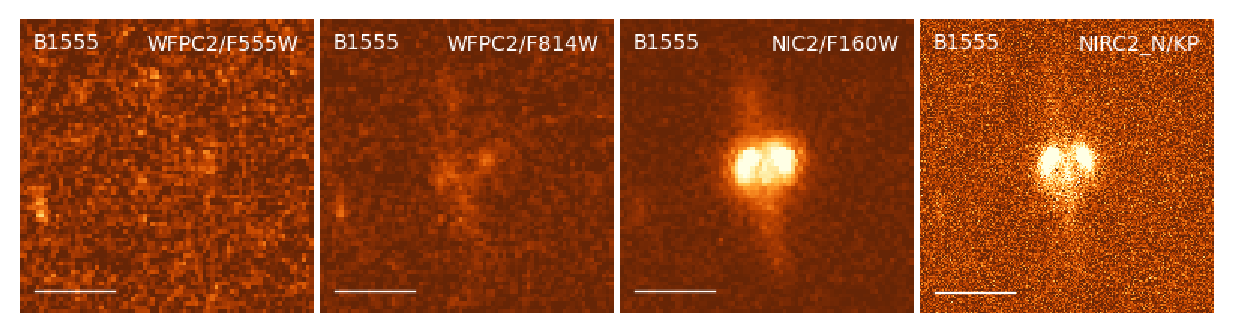
\includegraphics[width=0.95\textwidth]{B1555_gallery.eps}
\caption{High-resolution multi-band imaging of B1555+375 with {\it HST}/WFPC2 at F555W (left) and F814W (middle-left), with {\it HST}/NICMOS/NIC2 at F160W (middle-right) and with Keck adaptive optics at $K^\prime$-band (right). All of the panels are 3.7 arcsec on a side and the scale-bar represents 1 arcsec.}
\label{fig:multiband}
\end{figure*}

It was first suggested by \citet{Mao1998} that the flux-ratio anomalies observed in the multiple radio-loud images of lensed quasars could be interpreted as a sign of the presence of substructure in lens galaxies. Indeed, small perturbations in the gravitational potential are sufficient to cause flux-ratio anomalies in gravitationally lensed systems \citep{metcalf01,Dalal2002,Bradac02}, particularly for those systems with a close pair of merging images \citep{KD04}. At radio wavelengths, the lensed images are neither sensitive to micro-lensing from stars (\citealt{K03}; although see \citealt{koopmans00}), nor to dust extinction. Also, any variation in the properties of the radio images that are due to propagation effects (e.g. interstellar scattering or free-free absorption) have a well understood frequency dependence that can be identified and accounted for (e.g. \citealt{biggs03,M07,winn04}). This makes the flux-ratio anomalies of radio-loud lensed images a promising tool to detect and measure dark matter substructures in a large sample of distant galaxies \citep{Dalal2002}. However, a recent comparison of the observational data (eight gravitational lens systems with four or more images) with the predictions from a set of cold dark matter simulations that are representative of the mass and redshift of the lens galaxies suggests that there is only a 1--4 per cent probability that the full observed flux-ratio distribution is produced only by substructure \citep{Xu15}.

The \emph{gravitational imaging technique}, which alternatively utilizes the surface brightness distribution of extended arcs and Einstein rings to detect low-mass substructures within lensing haloes, was introduced by \citet{K05} and \citet{V09}. This method has given a measurement of the substructure mass fraction for a sample of 10 lensing galaxies that is currently in agreement with the theoretical expectations from cold matter matter simulations \citep{V14a,V12}. The reason for the conflicting results between the flux-ratio anomaly and gravitational imaging techniques is currently not clear.  While this could be the result of small sample statistics, it could also be an indication that the flux-ratio anomalies have a different origin than clumpy substructure \citep[see][for a discussion]{Xu15}.

%While this could be the result of small sample statistics, it could also be an indication that the flux-ratio anomalies have a different origin than substructure. 
 
In this letter, we explore the idea that not all flux-ratio anomalies are due to the presence of clumpy substructure, but that some originate from more complex lens galaxy mass distributions than have initially been considered. To this end, we use new infrared imaging data from the Strong lensing at High Angular Resolution Programme \citep[SHARP;][]{mckean07,lagattuta10,SHARP12, V12}. The main goal of SHARP is to investigate galaxy structure and other astrophysical topics through the re-observation of known gravitational lens systems at high angular resolution, making use of observations with (1) adaptive optics (AO) on the W. M. Keck telescope, (2) the {\it Hubble Space Telescope (HST)}, and (3) large radio and mm interferometric arrays. 

Here we focus on CLASS B1555+375 \citep{Marlow99}, which was discovered as part of the Cosmic Lens All-Sky Survey \citep{CLASS1,CLASS2}. B1555+375 has four lensed images with a maximum separation of 426~mas in a fold configuration.  The two merging lensed images show a strong and persistent flux-ratio anomaly at radio wavelengths, and previous radio monitoring observations ruled out microlensing effects as the cause of the anomaly \citep{K03}. As B1555+375 was included in the observational and theoretical analyses of both \citet{Dalal2002} and \citet{Xu15}, understanding its mass distribution is of key importance to assess any systematics with the inferred level of substructure in the lensing halo with the flux-ratio anomaly method. The SHARP imaging data are introduced in Section 2 and we present a revised lens model using these data in Section 3. The results of this analysis and their implications are discussed in Section 4. Note that the redshifts of both the lens galaxy and the lensed source are unknown for B1555+375, so we assume redshifts of $z_l = 1$ and $z_s = 1.5$, respectively, due to their red colours \citep{Marlow99}. This assumption has no effect on the derived magnifications or flux-ratios of our analysis.

\section{Observations \& Data reduction}

Our dataset consists of optical and infrared imaging taken with the W. M. Keck-II Telescope and HST, and high-resolution radio imaging taken with the Very Long Baseline Array (VLBA), which are discussed below and are summarized in Table~\ref{tab:obs}.

\subsection{Keck adaptive optics and {\it HST} imaging}

B1555+375 was observed as part of SHARP using the NIRC2 camera on the W. M. Keck-II Telescope on 2012 May 16 (PI: Fassnacht).  The AO system was used, with the corrections derived from the laser guide star and a $R=14.4$-mag tip-tilt star that was located $\sim45$~arcsec from the lens.  The narrow camera mode was used, giving a field of view of $\sim10$~arcsec on a side and a pixel scale of 10~mas. Six dithered 300~s exposures were obtained in the $K^{\prime}$-band filter.  The data were reduced with the standard SHARP pipeline, which is a python-based package that is a refinement of the process described by \citet{Auger_EELS1}.  A cutout of the final reduced image is shown in Fig.~\ref{fig:multiband} and also in Fig.~\ref{fig:merlin}, where the contours from 5-GHz Multi-Element Radio Link Interferometer Network (MERLIN) imaging by \citet{Marlow99} and 1.66-GHz VLBA imaging (see below) are overlaid.

B1555+375 was also observed with the {\it HST} in three broad bands.  The optical data were obtained with the Wide-Field Planetary Camera 2 (WFPC2) in the F555W and F814W bands (GO-8804; PI: Falco), while the Near Infrared Multi-Object Spectrograph (NICMOS) was used to observe the system in the F160W band (GO-9744; PI: Kochanek).  The NICMOS observations were obtained with the NIC2 camera.  We reduced all of the archival \textit{HST} data with the standard {\sc multidrizzle} pipeline, producing final drizzled images with pixel-sizes of 50~mas. The reduced images are also shown in Fig.~\ref{fig:multiband}. The lens and the lensed images are not detected at high significance in the optical bands, but are clearly seen in the NICMOS F160W image

There are several notable features in the high-resolution AO and {\it HST} data. These include the nearly complete lack of emission associated with lensed images B and D, as can be seen by comparing the radio contours to the $K^\prime$-band emission  (Fig.~\ref{fig:merlin}), and the faint, but clearly visible emission from what appears to be an edge-on lensing galaxy, with a position angle of $\sim 10$~deg and an ellipticity $e \sim 0.8$, where $e$ is defined in terms of the axis ratio $q$ as $q=1-e$.  We note that the position angle of the lensing galaxy is such that the disc emission lies close to the lensed images B and D. Therefore, the lack of emission that is seen from these images is likely due to dust extinction and additional demagnification due to lensing. 

\subsection{Very Long Baseline Array imaging}

B1555+375 was observed with the 10 telescopes of the VLBA at a central observing frequency of 1.66 GHz on 2000 March 21 (BN0009; PI: Norbury). The data were recorded at 128 Mbits~s$^{-1}$ and then correlated to produce two spectral windows with 8 MHz bandwidth, 16 channels and both circular polarizations (RR and LL). The observations were phase referenced using J1544+398 every 3 min over the total observing time of 3 h. The data were reduced in the standard manner using the {\sc vlbautlis} analysis pipeline that is part of the Astronomical Image Processing Software (AIPS). Imaging was done with the {\sc clean} algorithm in AIPS using natural weighting of the visibilities, and restored using an elliptical beam of size $9.7 \times 6.9$~mas at a position angle of $-7.6^\circ$ east of north. The final map (also shown in Fig.~\ref{fig:merlin}) has an rms of 78~$\mu$Jy~beam$^{-1}$.

We find that lensed images A and B have been resolved into a gravitational arc that is $\sim100$~mas in size. Image C is still compact on mas-scales, whereas image D is only marginally detected ($\sim6~\sigma$). We immediately see from the high resolution VLBA imaging that image B has a smaller angular size than image A, which is consistent with a perturbation in the mass model being responsible for the flux-ratio anomaly (recall that gravitational lensing conserves surface brightness), as opposed to free-free absorption or interstellar scattering.

\begin{table}
\centering
\caption{Summary of the B1555+375 observations.}
\begin{tabular}{llccc}
\hline
Telescope		& Camera			&  Band 		& Date				&$t_{exp}$ (s) \\
\hline
VLBA			&					& 1.66 GHz	& 	2000 Mar 21	& 10800\\
\textit{HST}	& WFPC2    		& F555W		&	2000 Oct 09	& 5200\\
\textit{HST}	& WFPC2    		& F814W		&	2000 Oct 09 	& 5200\\
\textit{HST}	& NICMOS/NIC2	& F160W		&	2003 Nov 02	& 5376\\
Keck-II			& NIRC2 AO		& $K^\prime$	& 	2012 May 16	& 1800\\
\hline
\end{tabular}
\label{tab:obs}
\end{table}

\section{Lens modelling}

The flux-ratio anomaly and relative sizes of the images at radio-wavelengths implies that there must be some form of perturbation to the gravitational lens mass model, which has thus far been attributed to dark matter substructure within the lensing galaxy or along the line of sight to the lensed images \citep{Dalal2002,Xu12,Xu15}. However, our high-resolution near infrared imaging suggests the intriguing possibility that the mass perturbation could be due to an edge-on disc component within the lens. To test this possibility, we model the system with a disc component in order to see if a plausible mass model can explain the flux-ratio anomaly without the need for additional substructure.

We use the lens modelling code {\sc gravlens} \citep{Kee01} to model the compact radio components. The inputs to the model are the observed image positions measured from the MERLIN radio observations of \citet{Marlow99} as all of the images are significantly detected in these data. The flux-ratio measurements are taken from \citet{K03}, who used half a year of MERLIN monitoring to obtain flux-ratio curves. In total, there are 11 constraints to the mass model provided by the observational data. As a first trial of modelling, we re-create the singular isothermal ellipsoid without external shear (SIE; 7 free parameters) model of \citet{Marlow99} to check the performance of a simple lensing potential. Consistent with previous studies \citep{Marlow99,Xu15}, a single elliptical potential model cannot reproduce the observed flux-ratios in B1555+375 (see Table~\ref{tab:results}). 
%; reduced $\chi^2 =97.3$

The next step is to test if a physically plausible edge-on disc can cause a perturbation in the strong lensing mass model that produces the observed flux ratio anomaly of  merging images A and B. An exponential disc profile best describes the disc component in spiral galaxies because it matches the light distribution \citep{Kee98}. We thus choose a SIE plus an exponential disc model (SIE+ExpDisc) in our study of B1555+375. The free parameters of the model are the SIE Einstein radius ($b$), centroid position, ellipticity ($e$), position angle ($\theta$), the exponential disc intrinsic central density ($\kappa_0$), and scale length ($R_s$). A detailed definition of these mass profiles is described by \citet{Kee01}. The source position adds two additional model parameters. We have not included a third component such as an external shear or an NFW halo because the number of constraints provided by the compact images detected by MERLIN is not sufficient to constrain such a model. Significantly deeper observations at a higher bandwidth with current very long baseline interferometric arrays can test more complex models in the future by imaging the extended gravitational arc and more significantly detecting image D. 

To obtain the best-fit lens model, we explore the parameter space with the following steps. First, we use the best-fit model of \citet{Marlow99} as the starting point for the SIE and exponential disc profiles. We add information from the Keck AO image for the disc, starting with an ellipticity of $e=0.8$ and a position angle of $\theta=10^\circ$.  All of the model parameters are then allowed to vary, but we fix the centroid positions of the SIE and exponential disc to the infrared positions with a Gaussian prior ($\sigma = 0.05 $~arcsec). The total number of free parameters is 13. After obtaining the best-fit lens model, we run a Markov-Chain Monte-Carlo (MCMC) analysis to explore the parameter space for the uncertainties.

The best-fit model parameters and 68\% CL errors are listed in Table~\ref{tab:model} and the lens model is illustrated in Fig.~\ref{fig:model}. Table \ref{tab:results} also shows the comparison between the observed radio data and the model-predicted image positions and flux ratios. We find that by adding an elongated exponential disc to a smooth SIE model there is significant improvement in the predicted flux-ratios when compared to the results for the SIE-only model. 
% with a reduced $\chi^2 = 2.7$
The positions are all in agreement, and the flux-ratios are consistent at the $2\sigma$ level, with excellent agreement now obtained for the two merging images A and B. The remaining differences in fluxes may due to the real lensed source being slightly extended rather than the point source that we used in our model. The model requires that the exponential disc component makes up about 10 per cent of the total mass within the Einstein radius (1.7~kpc for a lens redshift of $z_l = 1$), which is not unreasonable. We note that there is a significant 0.036~arcsec offset between the SIE and exponential disc components, which is likely due to an additional ellipticity in the model (e.g. from an external shear) that is being partly compensated for by the disc component. Again, more complex mass models that use the full extent of the gravitational arc and the compact lensed images from future high resolution radio imaging will be able to confirm this.

\begin{figure}
%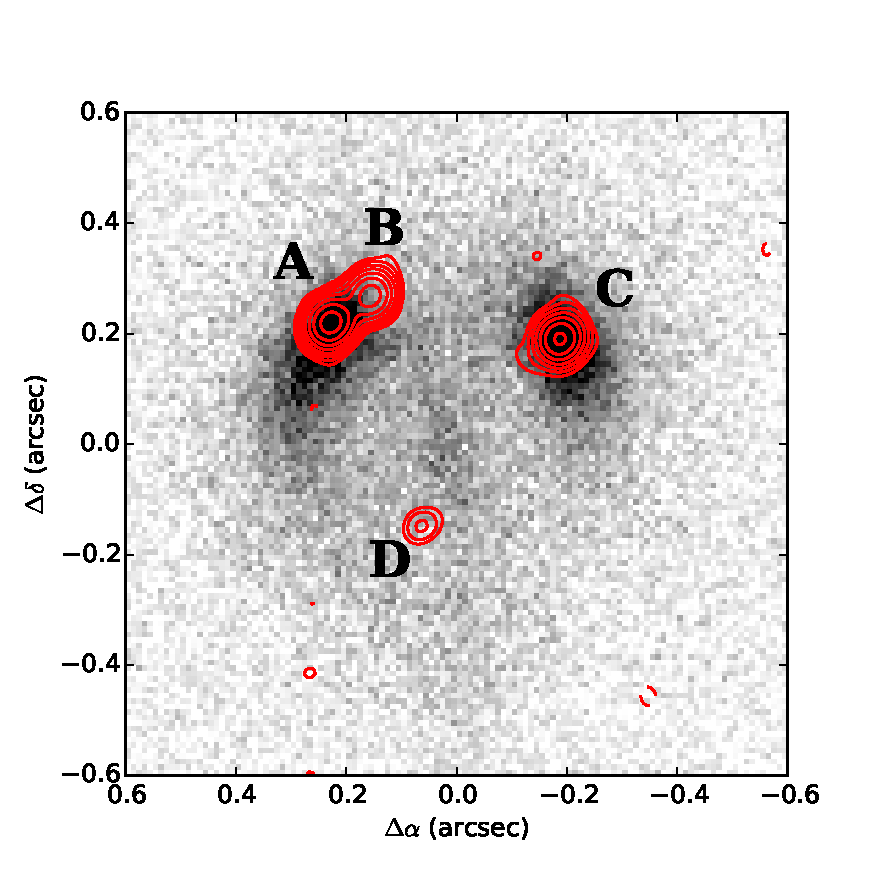
\includegraphics[width=84mm]{1555_ao_merlin_overlay.eps}
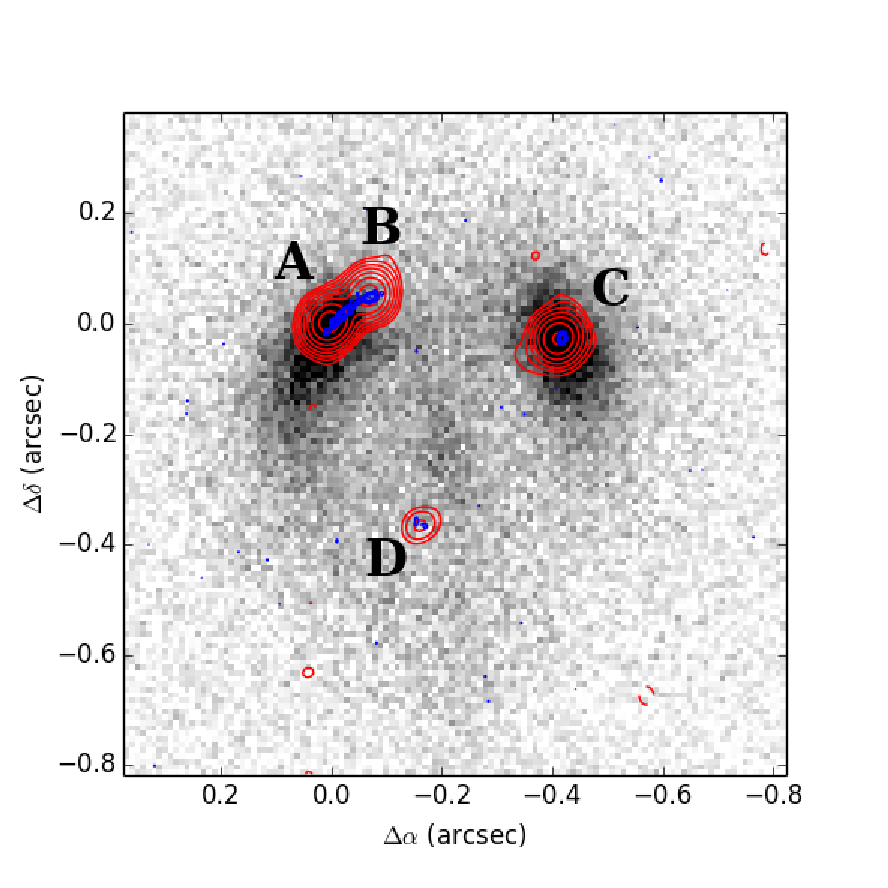
\includegraphics[width=72mm]{fig2_twocontour_b.eps}
\caption{High-resolution $K^\prime$-band imaging of B1555+375 with contours from the MERLIN observations (red) of \citet{Marlow99} and the VLBA observations presented here (blue) overlaid.}
\label{fig:merlin}
\end{figure}

\begin{figure}
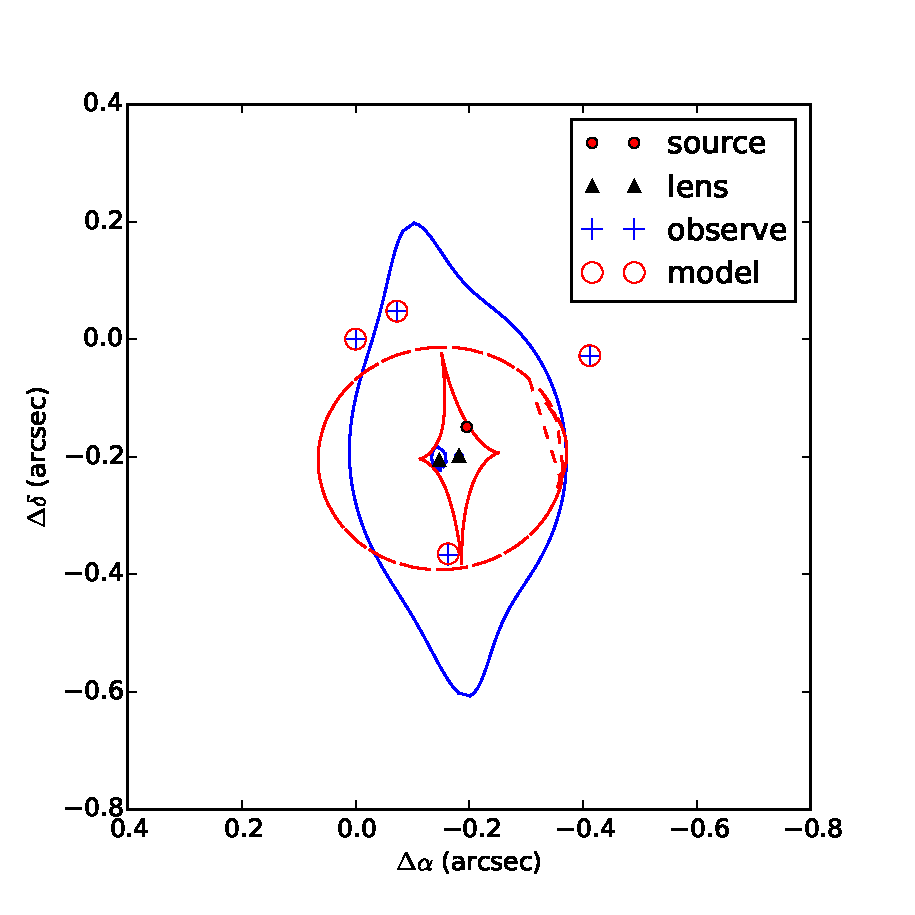
\includegraphics[width=72mm]{gravlens_exp_try5_plot.eps}
\caption{Observed radio (blue pluses) and model-predicted (red open circles) image positions of B1555+375. The lens-plane critical curves are shown with the blue solid line and the source-plane caustics are shown with the red dashed line. The position of the source is at ($-0.1953$, $-0.1494$), which is marked by the red filled circle. The centroid positions of the two mass components of the lens (an SIE and an exponential disc) are marked by the black filled triangles.}
\label{fig:model}
\end{figure}

\begin{table*}
\centering
\caption{A summary of the observational constraints and the predicted lens-model parameters. The lensed image positions in the radio \citep{Marlow99} (in arcsec) and average flux ratios \citep{K03} are respect to image A. Uncertainties in the position measurements for images A, B and C are $0.001$~arcsec and for image D are $0.006$~arcsec.}
\begin{tabular}{cccccccc}
\hline
Image	&\multicolumn{3}{c}{Observed MERLIN} 	 	& \multicolumn{4}{c}{Model-Predicted}\\
		&\multicolumn{3}{c}{5 GHz}		& & & {SIE+ExpDisc} & SIE-only\\
		&East &North & Flux ratio &East 	&North & Flux ratio &Flux ratio\\ 
\hline
A  &$0$    		&$0$			&  $1$ 				&$+0.000$  &$+0.000$	& $1$ 		& $1$\\  
B  &$-0.073$	&$+0.048$	& $0.620 \pm 0.039$ 	&$-0.073$ &$+0.048$		& $0.620$ 	& $0.971$ \\  
C  &$-0.412$ 	&$-0.028$	& $0.507\pm 0.030$	&$-0.412$ &$-0.028$		& $0.461$ 	& $0.312$\\  
D  &$-0.162$	&$-0.368$	& $0.086 \pm 0.024$ 	&$-0.163$ &$-0.365$		& $0.115$ 	& $0.106$\\  
\hline
\end{tabular}
\label{tab:results}
\end{table*}

\begin{table}
\centering
\caption{Best-fit model parameters and uncertainties for our two-component SIE + exponential disc lens model (our single SIE model is effectively equivalent to the model in \citet{Marlow99} and so is not shown here). The positions are measured in arcsec, relative to the radio position of image A. The ellipticity is defined as $e=1-q$ and the position angles are measured in degrees east of north. The Einstein radius $b$ and disc scale radius are measured in arcsec.}
\begin{tabular}{ccc}
\hline 
Parameter    & SIE Component & ExpDisc Component  \\
%   & (SIE) & (ExpDisc)\\
\hline
$\Delta$RA	& $-0.182 \pm 0.005$		& $-0.147 \pm 0.005$\\
$\Delta$Dec	& $-0.199 \pm 0.005$		& $-0.206 \pm 0.006$ \\
$b$ 			& $0.21 \pm 0.01$  		& $0.11 \pm 0.01$  \\
$e$	  		& $0.31 \pm 0.01$			& $0.87 \pm 0.01$ \\
$\theta$ 		& $3.0 \pm 0.6$			& $7.0 \pm 0.7$	 \\
$R_s$			& ...  						& $0.28 \pm 0.01$	 \\
\hline
\label{tab:model}
\end{tabular}
\end{table}


\section{Discussion \& Conclusions}

Although flux-ratio anomalies provide a powerful tool to investigate low-mass substructure in lensing haloes out to cosmological redshifts, it is clear that some care is needed in interpreting the results. It is now well established that observations of radio-loud gravitational lenses may provide the most robust observational constraints because they are less affected by dust extinction and microlensing, and monitoring can determine the best estimate of the intrinsic flux ratios. This has led to an oft-studied sample of eight radio-loud gravitational lenses with well-defined flux-ratio measurements \citep{Dalal2002,KD04,Xu15}. In general, lens models that are based only on the locations of lensed radio-loud images have large degeneracies due to the limited number of constraints that are provided by 50 to 200~mas imaging of the unresolved sources \citep[e.g.][]{Ka91}. Furthermore, observed flux-ratio anomalies may not be due exclusively to a population of low-mass "dark" substructures, as already seen in the MG J0414+0534 and MG J2016+112 systems, where there is evidence for luminous companion dwarf galaxies that can account for the observed flux ratios, and even observed astrometric anomalies (\citealt{ros00,chen07,more09}; see also \citealt{mckean07,jackson10}). 

Here, we find evidence for an edge-on disc in the flux-ratio anomalous gravitational lens B1555+375 that can also account for the required perturbation in the mass model. Such high-order deviations from a smooth mass distribution have already been suggested \citep{evans03,congdon05}, but this is the first time that a disc has been observed and modelled to account for a flux-ratio anomaly. However, it is important to realise that by including observationally motivated perturbations like luminous dwarf companions or edge-on discs in the mass models, we are still limited in our interpretation since we must assume that the anomalies are due exclusively to these additional components. For B1555+375, it may be possible to independently constrain the mass of the disc through kinematic measurements (most likely from mm-wavelength resolved emission line observations), which would test whether the disc makes a sufficient contribution to the mass model (e.g. as in the case of B1933+503; \citealt{suyu12}). Also, as we have shown here, B1555+375 shows evidence for an extended $\sim100$~mas gravitational arc at radio-wavelengths that crosses the edge-on disc. Further high resolution imaging with very long baseline interferometry will provide the observational constraints required to fully test whether the extended disc is sufficient to cause the anomaly. Nevertheless, before concluding that the flux-ratios in any given lens system are a result of substructure, it is critical to explore a range of smooth models that are informed by additional observations or to do a comprehensive analysis such as that conducted by \citet{Xu15}. Otherwise, the derived substructure fractions should be considered as upper limits.
 
Our results for B1555+375 clearly demonstrate that a lack of knowledge about the lens galaxy mass distribution, combined with the limited information provided by the position of compact lensed images, can lead to improper lens models and a misinterpretation of the origin of flux-ratio anomalies. While upcoming large-scale surveys with the Dark Energy Survey, Kilo-Degree Sky-VIKING, Square Kilometre Array, {\it Euclid}, and Large Synoptic Survey Telescope, are expected to deliver new large samples of gravitationally lensed quasars, in the near future the discovery of new systems using narrow-line quasar emission \citep{N14} will provide a new and invaluable statistical perspective on the current constraints based on flux-ratio anomalies. We stress, therefore, that one should be very careful when interpreting the nature of flux-ratio anomalies, as prior simple assumptions on the lens mass distribution may a significant source of bias. 

Our analysis shows that in order to derive a precise quantification of the substructure population and other properties from strongly lensed flux-ratio anomalies, it is crucial to have a careful estimation of non-substructure effects, such as galaxy discs and nearby massive satellites. In fact, even in the presence of substructures, the observed flux-ratio anomalies could be still affected by the complex structure of the lens galaxy. Finally, additional near-infrared AO imaging from SHARP shows that B1555+375 is not the only gravitational lens having a significant disc component detection in the lensing galaxy.  These gravitational lenses will be investigated in a future work, but the images alone strongly suggest that other systems may have similar links between flux-ratio anomalies and disc components.

\section*{Acknowledgments}
We are grateful to Dandan Xu for useful discussions. CDF and DJL acknowledge support from NSF-AST-0909119.  LVEK is supported in part through an NWO-VICI career grant (project number 639.043.308). The National Radio Astronomy Observatory is a facility of the National Science Foundation operated under cooperative agreement by Associated Universities, Inc. Based on observations made with the NASA/ESA Hubble Space Telescope, obtained from the data archive at the Space Telescope Science Institute. STScI is operated by the Association of Universities for Research in Astronomy, Inc. under NASA contract NAS 5-26555. Some of the data presented herein were obtained at the W. M. Keck Observatory, which is operated as a scientific partnership among the California Institute of Technology, the University of California and the National Aeronautics and Space Administration. The Observatory was made possible by the generous financial support of the W. M. Keck Foundation. The authors wish to recognize and acknowledge the very significant cultural role and reverence that the summit of Mauna Kea has always had within the indigenous Hawaiian community.  We are most fortunate to have the opportunity to conduct observations from this mountain.

\bibliographystyle{mnras}
\bibliography{reference.bib}



\bsp
\label{lastpage}

\end{document}
